\externaldocument{simulator}
In this section details about the software architecture used by the COMAN and WALKMAN robot is introduced. In particular, this details the engineering efforts undertaken in view of the DRC competition in the software and control side. 
These details include considerations about control algorithms on the simulated vs physical robot, the software API and tools of the \textbf{OpenSoT} framework and in general for middle to high level control, and observations about the global humanoid architecture with a particular attention to the practical details required to produce robust incremental improvements in medium-sized teams. We also show a large set of examples of high-level task implementations as well as tests to evaluate the tooling against regressions, and in particular to test \textbf{OpenSoT}'s tasks, constraints and stacks (the highest level layer of the architecture which is automatically tested).
This set of tests and examples demonstrate the performances of the architecture and the easiness of writing complex sets of tasks and constraints in the OpenSoT framework.

\section{Development Pipeline}
Part of the engineering work on the hardware and software for the DRC competition entry of the WALKMAN robot involved organizing the efforts of a big team working under high pressure and delivering results in a very short amount of time.
During one year and a half, a whole robot has been built from scratch, together with a new simulator, low level joint control, a high level control framework, a software component model and UI for teleoperation.

This work has been coordinated across IIT and two more universities in the consortium (Univerity of Pisa - UNIPI and Universit\`e Catholique de Louvain - UCL). Part of the work needed to feature such an achievement has involved adopting a shared development workflow, and in particular, an automated build system.

The \emph{YCM} framework developed by the iCub facility department has been used for the WALKMAN project, which allows to automatically manage the build order, the automatic downloading, compilation and installation of dependencies and the management of versions for each separate module in the build, and integrates seamlessly with the ROS build system, either \emph{rosbuild} or \emph{catkin}.
The system allows to automatically install all the dependencies (binary or from source), to download, compile and install all the external libraries and the DRC modules in less than an hour, with a list of around $60$ modules managed automatically. It allows to specify a profile (i.e. \emph{ROBOT} and \emph{SIMULATION} depending on the target location for the installation, be either a control computer or a development computer, where algorithms need to be tested in simulation - the different choice automatically sets up the environment to synchronize the algorithm's clock either with a wall clock or simulation clock \label{sec:simulation_clock}) and interest focus (allowing to automatically disable compilation of unneeded packages based on the user focus, be either control, sensing, robot model development, architecture and networking). The build system is well documented and provides a set of scripts that have been found to be of use to the team (e.g. setting up environment variables to use a remote simulation server, setting up a networked control architecture with a remote ROS or YARP master servers, install daemons to automatically install services useful for simulation servers or control computers, and advanced version management utilities which allow to bulk branch, tag/freeze, and analyze the version and changes on all the modules managed by the build system). Lastly, it allows for bulk version management via branching of the build system itself: in fact, the configuration file specifying the desired branch or tag to use for all the modules managed by the build system (\texttt{cmake/ProjectsTags.cmake}) is versioned itself. This allows to easily generate \emph{versions} for the whole system, i.e. freeze notable working versions,  such as a system used for a demo, or a system tuned with a certain network architecture, or with a certain version of the robot, or eventually even to manage codebases tuned for a partial robot build (as mentioned earlier, e.g. in the case for parallel development of lower-body and upper-body of a humanoid robot).
A stripped-down version of the build system used for the DRC by the WALKMAN team is hosted online \cite{robotology-superbuild}, and is being used as a basis for other projects in the team. Its documentation is available \cite{robotology-superbuild-handbook} and is based on the original handbook developed for the team during the DRC.

The second fundamental aspect related to streamlining development and increasing productivity has been that of adopting a development workflow based on a series of fundamental steps:
\begin{itemize}
 \item a very large set of unit and integration tests, especially for the core libraries and the high level control libraries. Regression testing has been a fundamental tool to quickly develop a consistent set of algorithms that evolved during time
 \item a continuous build system
 \item a shared GIT workflow with \emph{master}, \emph{devel} and \emph{feature} branches, plus branches for each sprint (a so-called Agile development practice), or so called \emph{sprint-week} that got merged at the end of each sprint
\end{itemize}
The GIT distributed source code managament system has been used on a self-hosted \emph{gitlab} environment, which seved also as a hub for managing collaboration, by providing features for issue-tracking, code reviewing and documentation sharing via its WIKI system.

\section{Component Model}
In order to facilitate module development, a basic compoment model has been developed, the \emph{Generic Yarp Module} ( \emph{GYM}), based on the YARP framework.
Quoting its webpage ~\cite{GYM}, \emph{the Generic YARP Module (GYM) is a component model to easily develop software modules for robotics leveraging the YARP ecosystem}.
It makes use of the \emph{paramHelp}~\cite{paramHelp} library, which was designed to simplify the management of parameters of YARP modules and allows networked logging, configuration and (on-the-fly) reconfiguration. The library has been extended to automatically generate GUIs for online gain tuning. GYM also provides facilities for automatic module creation, were several templates (or skeleton) can be chosen, i.e. helper modules (for developing robotics tools), modules for robot control (for developing robotics control and sensing algorithm that need need to run periodically and with a fixed rate, and need to directly access a part or the entirety of the robot hardware) and generic modules (for developing robotics library that don't need to access directly the robot hardware but are still periodic, e.g. trajectory generators and state machines). 

\begin{figure*}[!ht]
\centering
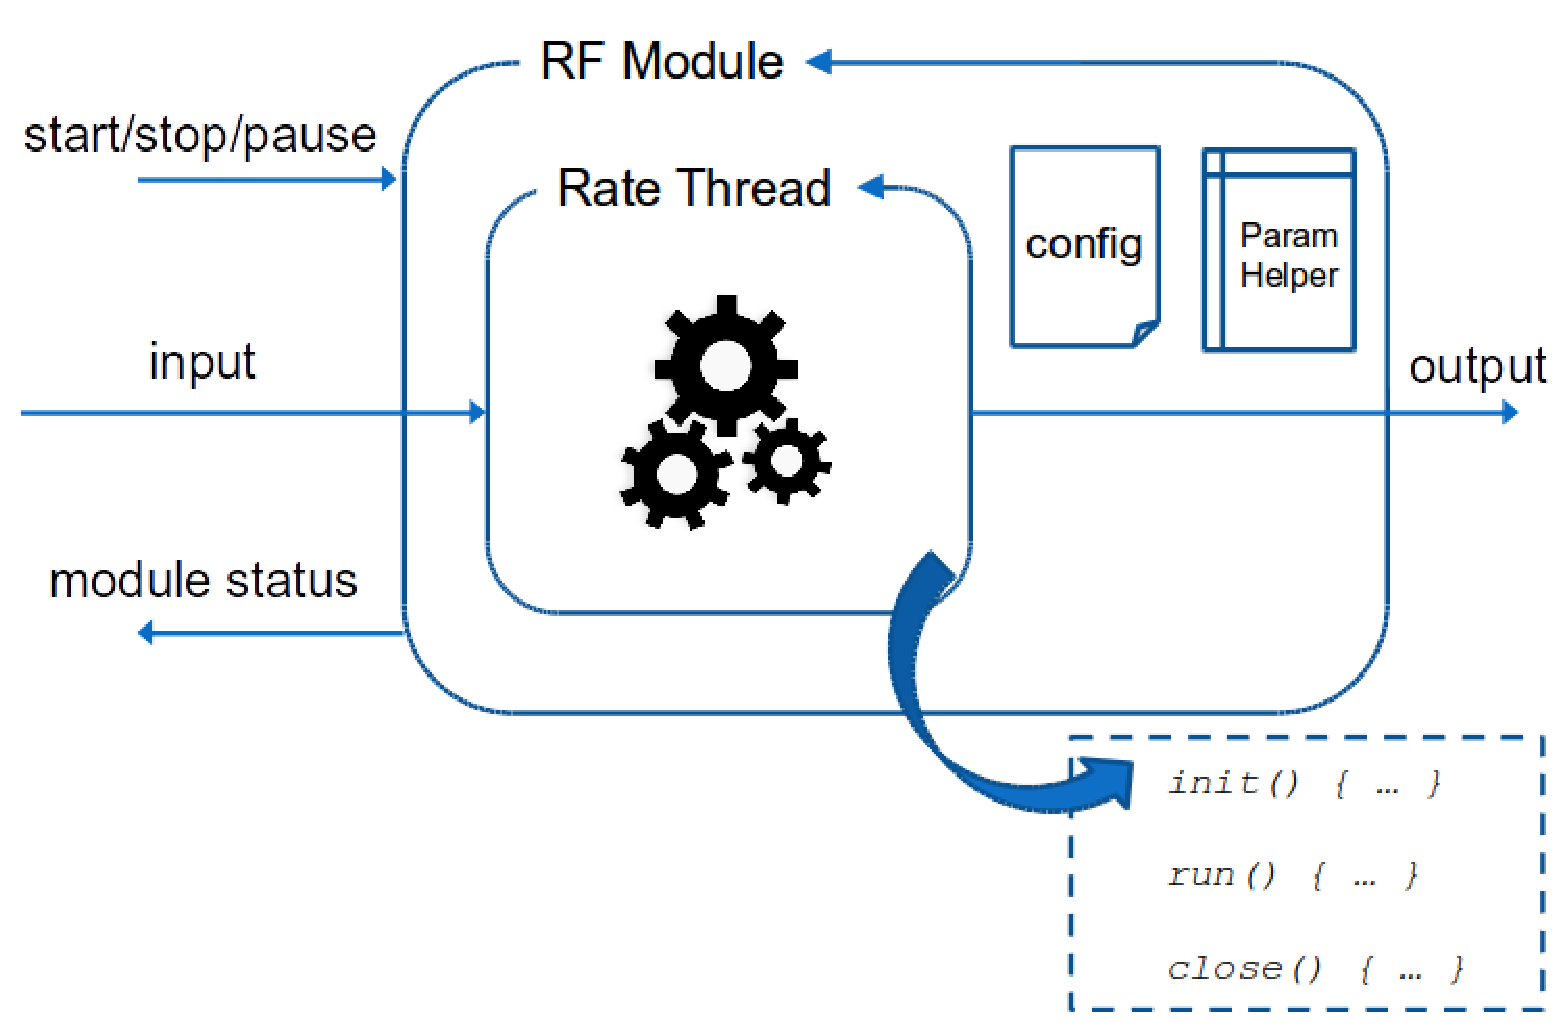
\includegraphics[width=0.7\textwidth]{images/GYM}
\caption{structure of a GYM module}
\label{gym}
\end{figure*}

Every module is composed of at least two threads.
A low frequency thread accepts high level management commands to \texttt{start}, \texttt{stop}, \texttt{pause}, \texttt{resume} execution of a module (the \emph{switch} interface), gives information on the status of the module (the \emph{status} interface), and provides a set of commands related to the \emph{paramHelp} that allow to view, set and eventually store to disk all of the module's algorithms parameters. 
Additionally, each module has a main thread that is specific to the kind of module to implement and is usually a high frequency thread that takes care of the control and obtains sensor feedback from the robot and task level commands by the user.

\section{Simulating and Controlling Compliant Robots}
The simulator is a fundamental part of the framework and the robot software development cycle as the first step to validate algorithms, thus minimizing the risks of hardware failures.
In these frameworks, the \emph{simulator} is a module that represents the real robot at the interface level (Figure \ref{yarp_simulation}). Such simulator module accepts control input (desired joint torques, desired joint position, ...) and outputs sensory feedback (cameras, joint positions, ...) from the simulated world. These simulators usually allow to have the human in-the-loop permitting to train a human operator. The most important aspect is that they allow to develop modules that directly will work in the real robot without any need to rewrite code. In fact, when the real robot is used, there is a module that replaces the simulator by providing the same hardware interfaces. 

With these concepts in mind we decided to extend one of the most known robotics simulator, Gazebo (\cite{koenig2004design}), to be compatible with one of the most used robotics framework, YARP (Figure \ref{coman_icub_gazebo}), developed in the Italian Institute of Technology. 
YARP is supported by the iCub simulator (iCubSim, \cite{Tikhanoff:2008:OSC:1774674.1774684}) that is dedicated to a specific platform. The needs of a more generic tool for simulating different robots rise up. 
Gazebo, which has been recently chosen as the simulator for the DARPA Virtual Robotic Challenge (VRC, \cite{DRC}), allows the use of different dynamic engines, it is easily expandable through plugins and it has a strong and active community. Gazebo is maintained by the Open Source Robotics Foundation (\cite{OSRF}).

\label{structure}
It is useful to understand Gazebo plugins and YARP device drivers before describing the structure of our plugins (from now on \emph{gazebo\_yarp\_plugins}).

Gazebo plugins are C++ classes that extend the functionalities of Gazebo, while YARP device drivers are C++ classes used in YARP for abstracting the functionality of robot devices.
Usually, each class of gazebo\_yarp\_plugins embeds a YARP device driver in a Gazebo plugin. 

{\bf Gazebo Plugins}
A plugin is a piece of code compiled as a shared library and inserted into the simulator. A plugin has direct access to all the functionalities of Gazebo from the physics engine to the simulated world. Furthermore, plugins are self-contained routines that are easily shared and can be inserted and removed from a running system. There are 4 types of plugins in Gazebo: \textbf{world}, \textbf{model} and \textbf{sensor} plugins are attached to and control a specific simulated world/model/sensor respectively, while \textbf{system} plugin is specified on the command line and loads during the Gazebo startup.


{\bf YARP \emph{Device Drivers}}
YARP provides special devices that act as network proxies and make interfaces available through a network connection. This allows accessing devices remotely across the network without code change.

A device driver is a class that implements one or more interfaces. There are three separate concerns related to devices in YARP:
\begin{itemize}
\item Implementing specific drivers for particular devices
\item Defining interfaces for device families
\item Implementing network wrappers for interfaces
\end{itemize}
For example the Control Board device driver implements a set of interfaces that are used to control the robot (IPositionControl, ITorqueControl, etc.) and another set of interfaces to read data from the motors (IEncoders, etc).

\subsection{Gazebo-YARP Plugins}
The gazebo\_yarp\_plugins is made of:
\begin{itemize}
    \item Gazebo plugins that instantiate YARP device drivers,
    \item YARP device drivers that wrap Gazebo functionalities inside the YARP device interfaces.
\end{itemize}

\subsection{Robot and Simulation Description Formats: URDF, SRDF, SDF}
Gazebo uses an XML-style format, Simulation Description Format (SDF), to save and load information about a simulated world or model. An SDF encapsulates all the necessary information for a simulation including the robot models, physics engin parameters, and plugins to be loaded (e.g. sensors plugins).


\section{Whole-Body Control}
\begin{wrapfigure}{r}{0.35\textwidth}
  \begin{center}
    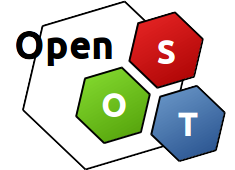
\includegraphics[width=0.25\textwidth]{images/openSoT_stickers}
  \end{center}
  \caption{OpenSoT Logo}
\end{wrapfigure}
Despite the existence of many control libraries for robotics, most of them are complex piece of software that rely on legacy code, and not easy to use for the final user. Furthermore, considering in particular the case of Inverse Kinematics (IK) frameworks, they are provided with a small set of implemented tasks and constraints. These problems make the typical IK framework a tool for just experts, ignoring the needs of a generic user who is in need of writing tasks for a complex robotic system. This work is a complement to \cite{rocchimingo:16} where the software API and tools of \textbf{OpenSoT} are presented. One of the major difference of \textbf{OpenSoT} framework with respect to other existing frameworks is the idea to \emph{collect} a comprehensive library of implemented tasks, constraints and solvers that the end-user can employ. Furthermore, the possibility to write their own tasks, constraints and solvers permits to easily enrich the existing set. This characteristic allows also to benchmark the performance of different IK problems formulations and different solvers for the same high-level tasks. 

A particular attention has been put also on the \emph{toolset} that has been developed and made available together with the library: visual markers for the Cartesian control, bindings for different programming languages, auto-generation of capsules model for the Self Collision Avoidance (SCA) constraint, a Math of Task description language and an utility library, \emph{iDynUtils} which takes care of wrapping several common robotics libraries to provide an easy-to-use comprehensive framework for robotics control (convex hull computation, self-collision checking, \emph{SE3} math). 

In this paper we also present a large set of tests and experiment to show how the framework can be used for many different high-level tasks such as walking, manipulation and interaction with the environment. We also consider different robots (simulated and real hardware) that intend to demonstrate how the library is robot agnostic.

The paper is structured as follows: in \textbf{\nameref{sec:software_architecture}} the basic API and tools are introduced, in \textbf{\nameref{sec:examples}}physical hardware and simulated  experiments are presented, and finally in \textbf{\nameref{sec:conclusions2}} some final considerations on the presented work are provided.

\subsection{OpenSoT Software Architecture}
\label{sec:software_architecture}
Designing a good Software Architecture has been a crucial step in the development of \textbf{OpenSoT}. Firstly, the design has been focused on requirements of agile programming as commanded by the tight schedules of the development for the DRC competition. The software should be straightforward to install and to use, be robust both algorithmically and at the implementation level, and allow for ease of extendability, reusability and integration with existing frameworks.

\subsubsection{Application Programming Interface (API)}
The \textbf{OpenSoT} API is structured to favor reusability.
Tasks are implemented through the class \emph{Task} which provides an interface to obtain $\A$ and $\b$, a weight matrix $W$ and a scalar weight $\lambda$ for the task (\texttt{\small getA()}, \texttt{\small getb()}, \texttt{\small getWeight()}, \texttt{\small getlambda()}).
Constraints and bounds are implemented in \textbf{OpenSoT} through the class \emph{Constraint} which implements a simple interface providing equality constraints (\texttt{\small getAeq()}, \texttt{\small getbeq()}), inequality constraints (\texttt{\small getAeineq()}, \texttt{\small getbLowerBound()}, \texttt{\small getbUpperBound()}) and bounds (\texttt{\small getLowerBound()}, \texttt{\small getUpperBound()}).

Both \emph{Task} and \emph{Constraint} classes have a pure virtual \texttt{\small update()} method to be implemented. Most of the kinematics and dynamics information are directly available inside the \emph{Task}/\emph{Constraint} thanks to a pointer to the model of the robot. The robot model (see \nameref{sec:idynutils} section) has to be updated at every control loop with measured joint position, velocities and force/torque, before the update of the IK problem as shown in Figure \ref{update}.

\begin{figure*}[!ht]
\vspace{2 mm}
\centering
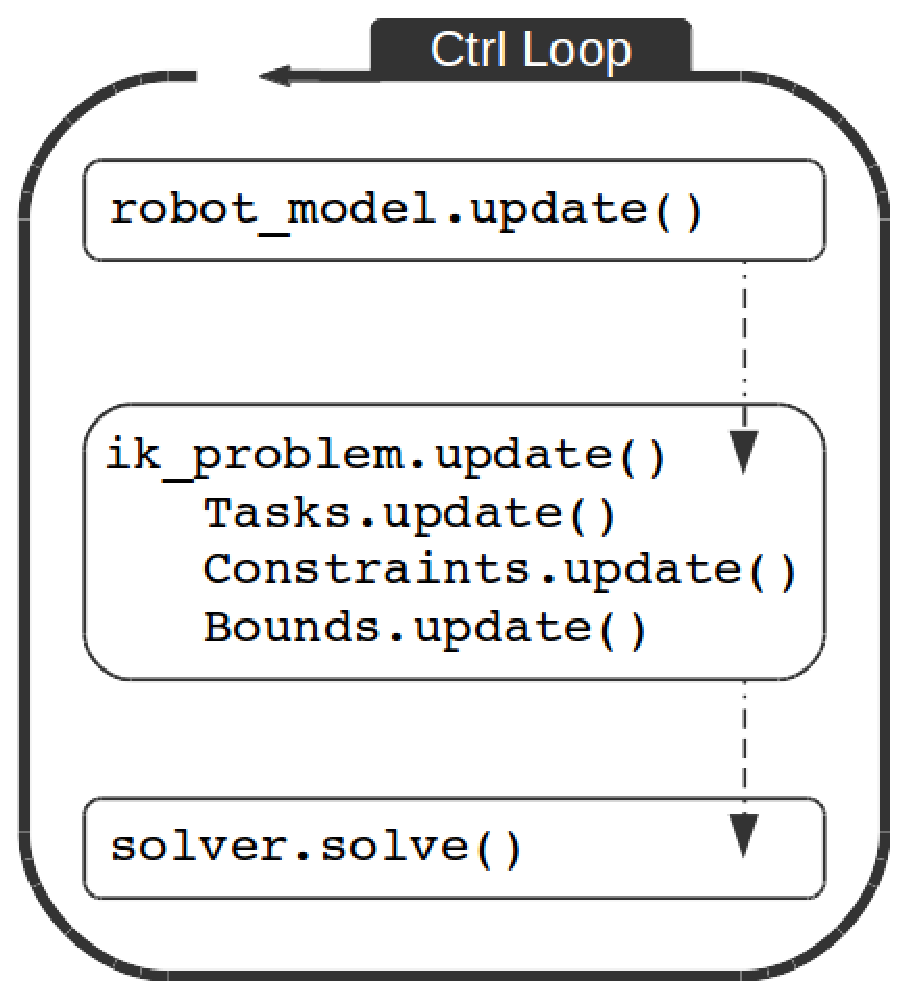
\includegraphics[width=0.25\textwidth]{images/software/update.eps}
\caption{At each control loop the robot model and the IK problem are updated and then the solver is called}
\label{update}
\end{figure*}

Controlling a new robot with \textbf{OpenSoT} requires only writing a new stack. Thanks to \nameref{sec:idynutils}, every robot which is provided with an \emph{URDF} and \emph{SRDF} can be imported for use with the library.

\textbf{OpenSoT} provide also a simple base class to write a \emph{Solver}. The main pure virtual methods consists in three constructors, depending if the solver permits to handle also bounds and constraints, and the \texttt{\small solve()} method. 

\subsubsection{Integration with Robotic Frameworks}
\label{sec:integration_with_robotic_frameworks}
By writing proper task wrappers it's possible to encapsulate the API and export the functionalities of \textbf{OpenSoT} over the network. Some wrappers are already available for the \emph{ROS} and \emph{YARP} frameworks. In particular, for \emph{ROS} the Cartesian and joint postural tasks are wrapped so that it is possible to perform simple tele-operation  through \emph{rviz}'s \emph{interactive markers}, as shown in Figure \ref{opensot_interactive_markers}.
\begin{figure*}[!ht]
\vspace{2 mm}
\centering
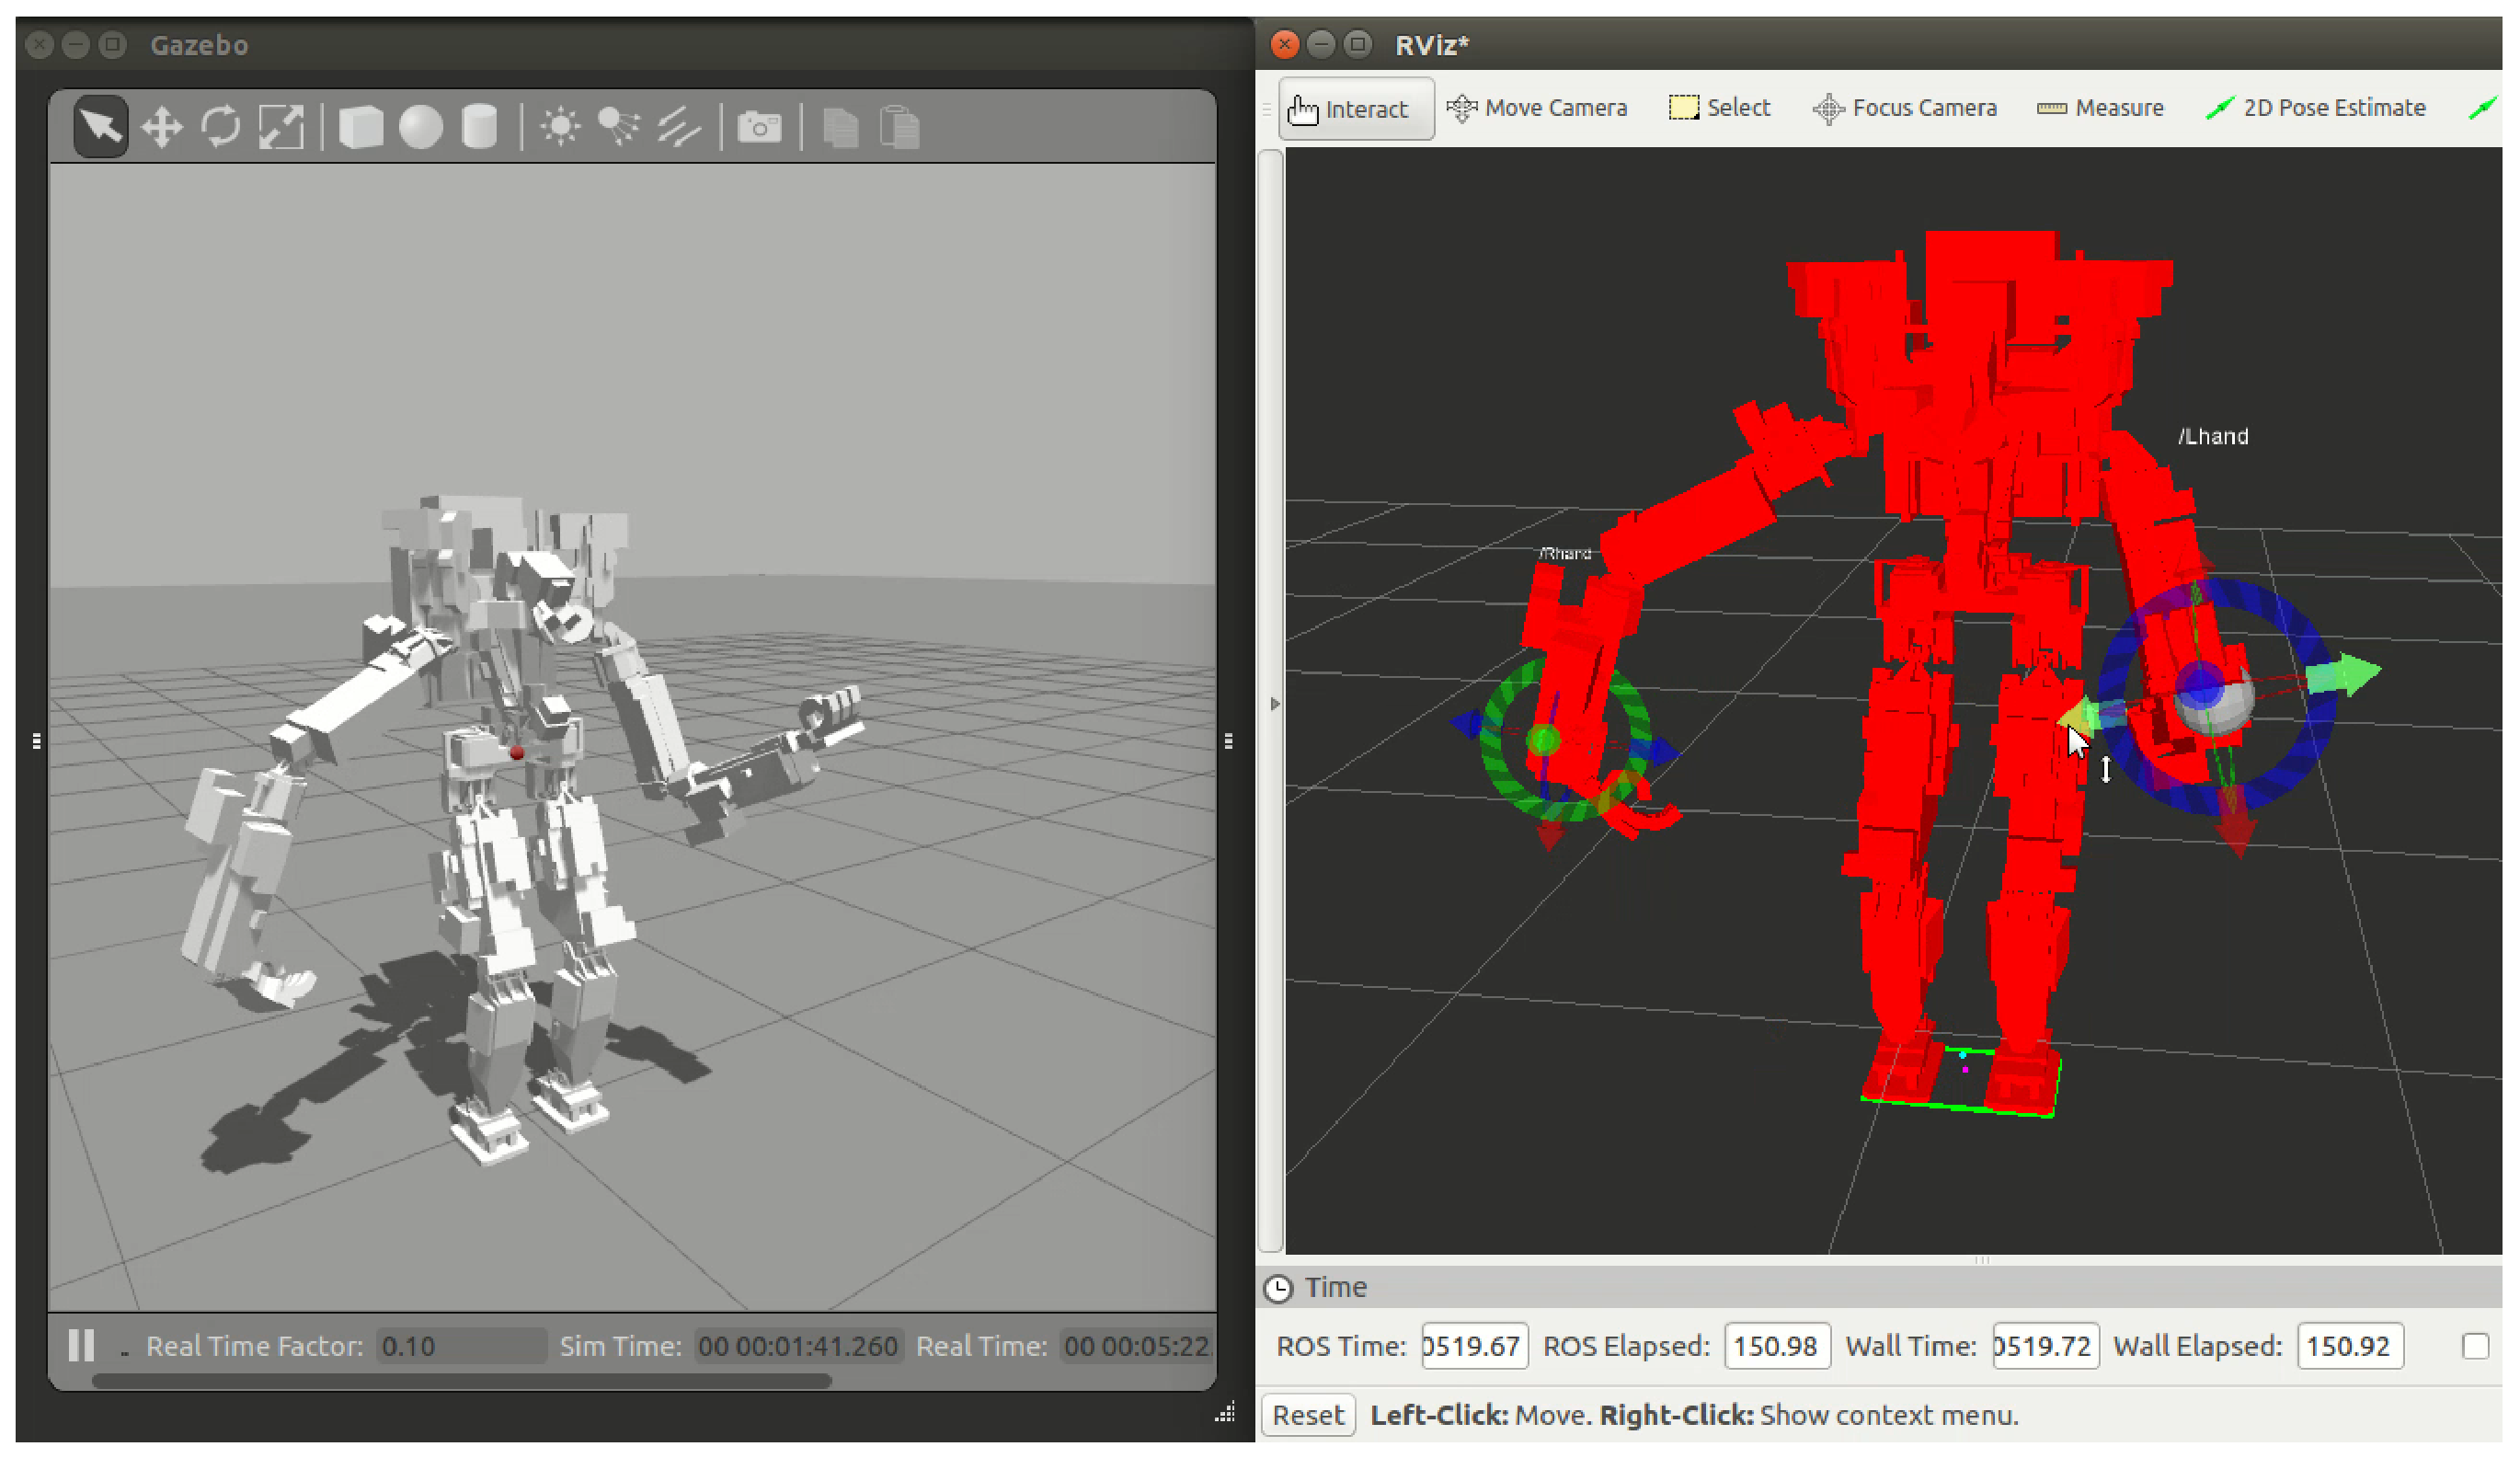
\includegraphics[width=0.7\textwidth]{images/software/hydra_tele_operation.eps}
\caption{The HYDRA robot tele-operated in simulation.}
\label{opensot_interactive_markers}
\end{figure*}
Through \emph{YARP} it's possible to change the parameters of all the tasks, including $\beta$ and $\W$, and to get and set the task reference when contemplated (e.g., Cartesian, CoM, postural).

\subsubsection{iDynUtils}
\label{sec:idynutils}
\todo{add a section about RobotUtils}

As a support library to the \textbf{OpenSoT} framework we developed a whole-body control library named \emph{iDynUtils}.
This library is responsible for loading the model of the robot via the \emph{iDynTree}\cite{Nori2015-zb,Nori2015-db} library.

The library is an interface and wrapper to other robotics libraries, and provides the following functionalities:
\begin{itemize}
\item robot pose estimate w.r.t. the world via forward-kinematics based dead-reckoning
\item loop closures/kinematic constraints via kinematic tree rebasing, e.g. foot switching
\item convex hull computation via \emph{PCL}, management of link is contact with the environment with frictional constraints
\item collision and self-collision checking via \emph{Moveit!} and \emph{fcl}, helper utilities to define collision white-lists, simplified bound in volumes support (capsules management)
\item Cartesian utilities for \emph{SE3} math, in particular quaternion implementation of (17) in \cite{rocchimingo:16}%\ref{eq:cartesian_error}
\item interfaces for automatic transformation of frame of reference/poles for force/torque readings, and for frame of reference of IMU readings
\item utility functions for management of the kinematic tree as a tree or as as a list of chains
\end{itemize}
In particular with respect to item 1, 2 and 3, the structure of the library makes so that the dead-reckoning is a simple integrator based on the forward kinematics of the robot.
In particular, among the links in contact with the environment, we select a link which will be called the  \emph{anchor} for the dead-reckoning phase, and a link to which the \emph{floating base} will be attached. While the computation of the IK problem's solution can take into account explicitly the virtual joints of the floating base, most of the tasks already implemented in \textbf{OpenSoT} will follow an approach where the Jacobians are cut to take into account only the actuated joints. In this way, the solution of the problem will be computationally less intensive as the Hessian of the equivalent QP problem will be smaller, and we will drop the chain-closure constraint (i.e., imposing that the chain going from the \emph{anchor} link to the world through the floating base virtual chain will have only internal movements, or alternatively, the twist of the \emph{anchor} link with respect to the world frame will be $0$). For this reason, the \emph{iDynUtils} library has been implemented to provide functionalities for both use cases, and in particular the \emph{anchor} and \emph{floating base} links can be coincident, and during a typical walking phase, they will switch from one support foot to the other (with the switch command given by the walking algorithm), and remain constant during the double support phase.

\subsubsection{Python Bindings}
A set of bindings is provided for the \textbf{OpenSoT} framework that allow to send commands to an existing stack that runs as a server. While the stack needs to be defined and compiled in C++ at the moment, the approach allows to program the tasks in python using simple interfaces. In particular, python interfaces are available to allow the creator of python clients for the \emph{YARP} bindings (introduced in \ref{sec:integration_with_robotic_frameworks}) to \textbf{OpenSoT}. The python bindings ease the process of creating messages for the \emph{YARP} interfaces, namely \texttt{pose} messages, \texttt{twist} messages, \texttt{joint position} messages and \texttt{trajectory} messages. Using these, the \texttt{YTask} python binding defines a generic binding to a task with a \emph{YARP} interface (a \emph{YTask}), such as getting and setting weights and gains. The \texttt{CartesianTask}, \texttt{CoMTask} and \texttt{PosturalTask} extend the base class \texttt{YTask} to provide specific functions to set and get references for the corresponding \emph{YARP} interfaces to the corresponding tasks, as written in C++ (see Figure \ref{fig:python_binding} for details).
An example is provided to generate generic bindings via \emph{SWIG} for interfacing with the \emph{Klampt} simulator.
\begin{figure*}
\vspace{2 mm}
\centering \includegraphics[width=0.6\textwidth]{images/software/python_markers.eps} 
\caption{Integration of Python and RVIZ markers inside \textbf{OpenSoT}} 
\label{fig:python_binding}
\end{figure*}


\subsubsection{Integration with Generic Simulators}
While \textbf{OpenSoT} has been used extensively with Gazebo, using an abstraction infrastructure that allowed to seamlessly switch from the physical robot to the simulated robot \cite{hoffman2014yarp}, the \textbf{OpenSoT} library is generic and can be used with any simulation and control infrastructure.
A suggested workflow for using \textbf{OpenSoT} with simulators and controllers written in C++ and python is provided in the examples. While the library \nameref{sec:idynutils} is model-based, and the model is populated using URDF and SRDF descriptions of a robot, the main steps for connecting the library to a generic software is to specify conversion functions to transform joint positions and references between the simulator and the \textbf{OpenSoT}-based controller.
The suggested way consists in transforming the joint reading vectors specified by the simulator in a joint readings map that associates the joint names with joint values, in a similar way to what \emph{ROS} enforces via joint state messages and \emph{YARP} implicitly does in the \emph{Gazebo YARP plugins}. The same is done in \textbf{OpenSoT} to transform the joint readings map into its joint readings vector (in general the two vectors might assume different joint indices). Once specified this lightweight translation layer that uses sensors names to exchange data, \textbf{OpenSoT} can be encapsulated in the custom simulation/controller architecture. An example of a \emph{HUBO} robot being simulated in the \emph{Klampt} simulator is shown in Figure \ref{fig:HUBO}, where the stack for the three tasks is a whole body stack composed of
\begin{equation}
\begin{pmatrix}

\left(T_{\substack{\text{Right}\\\text{Foot}}} + T_{\substack{\text{Left}\\\text{Foot}}}\right)\setminus\\
\\
T_{\text{CoM}_\text{XY}}\setminus\\
\\
T_{\text{Waist}_\text{Z}}\setminus\\
\\
\left(T_{\substack{\text{Right}\\\text{Wrist}}} + T_{\substack{\text{Left}\\\text{Wrist}}}\right)\setminus\\
\\
T_{\substack{\text{Joint}\\\text{Postural}}}

\end{pmatrix}
<< \left(B_{\substack{\text{Joint}\\\text{Limits}}} + B_{\substack{\text{Joint Velocity}\\\text{Limits}}}\right)
\end{equation}
and velocity allocation strategy (see \nameref{velocity_allocation}).
The Hubo robot used in the simulation has a $1$ DoFs torso, $6$ DoFs legs and arms, $2$ DoFs neck, $15$ DoFs arms. Figures \ref{fig:HUBO} are generated by using \emph{Gazebo}. Notice how the two simulators use a different approach to controller simulation, whereas in \emph{Klampt} we have a synchronous execution of the controller together with the simulator, while in \emph{Gazebo} the controller runs asynchronously and needs to be synchronized by using the simulation clock, so as to obtain a simulated real-time execution on the controller.

\subsubsection{Notes on Robustness}
The \textbf{OpenSoT} framework has been developed with stability and robustness in mind, both at the algorithmic level, and at the software level. Best practices for software development are crucial when working in big groups of people under a tight deadline. For this reason, a set of unit and integration tests has been developed, which where possible also generate simulation data and graphs for human inspection. On the debugging side, the solver dumps the QP problem stack once a failure in solving the a problem is encountered, which allows for inspection and reproduction.

\subsubsection{Utilities}
Other than the \nameref{sec:idynutils} package, several utilities have been developed as \textbf{OpenSoT} ancillaries. Between these, the \nameref{subsub:CapsuleGeneration} toolkit and the \nameref{subsec:Previewer} class. The former allows to generate simplified bounding volumes for the robot links' geometries, as required by the collision avoidance task as defined in section Self-Collision Avoidance Constraint in \cite{rocchimingo:16}. %\ref{sec:collision_avoidance}.
The latter allows to automatically check for a defined motion before executing it on the robot, by kinematically simulating a certain task while checking user-defined convergence and maximum error thresholds, and checking for self-collision. In particular, the \nameref{subsec:Previewer} is implemented to so be used programatically to generate a Task workspace for a given stack and robot.

\paragraph{Capsule Generation}
\label{subsub:CapsuleGeneration}
In order to compute the minimum distance between links, an automated way to generate capsule approximation of meshes for URDF model is needed. To this extent, we developed tools using the \emph{Roboptim} \cite{Moulard2013-nk,Moulard_undated-tm} numerical optimization for robotics library. Through the plugin \emph{roboptim-capsule} the library finds the minimum volume capsule that contains the given polyhedra. The optimization problem resolving in optimal capsules is reported here for convenience \cite{el_khoury2013-rp}

\begin{eqnarray*}
\min_{e1,e2,r} & \left\Vert e_2 - e_1 \right\Vert_2 \pi r^2+\frac{4}{3}\pi r^3\\
{s.t.}  & r-d(p,e_1e_2) \ge 0, & \vee p \in P
\end{eqnarray*}

where $p$ is a vertex of the polyhedron $P$ and we want to find the capsule of minimum volume for which the distance $(p,e_1e_2)$ between $p$ and the segment $e_1e_2$ is smaller than the capsule radius.

The integration of the plugin with our architecture needs to circumvent the lacking of the capsule primitive in the URDF format and on all the ecosystem of libraries using the URDF format, including the popular interface \emph{rviz}.
Once our wrapper analyzes the URDF file of the model described with meshes, it will convert them to the corresponding capsules via the \emph{roboptim-capsule} optimization, and create an URDF file with cylinders in place of meshes. The wrapper takes care to transform the capsule parameters between the endpoints-radius representation and radius,length,center representation during the process, in order to integrate the different components of the system.
The self collision avoidance constraint then will scan the URDF looking for cylinders and interpret them as the body of a capsule, to feed the \emph{fcl} library which takes care of computing minimum distances between the robot links using the simplified bounding volume. 
An example of application of this method on different robotic platforms can be seen in Figure \ref{fig:capsules}.
\begin{figure*}
\vspace{2 mm}
\centering 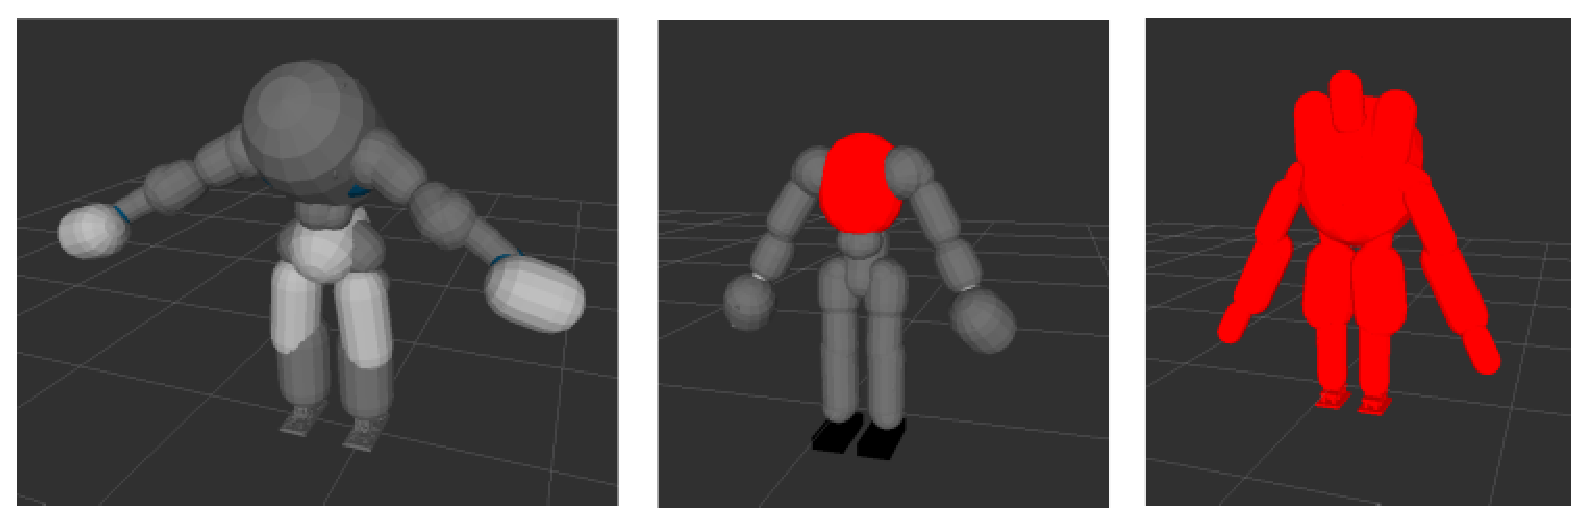
\includegraphics[width=0.8\textwidth]{images/software/robots_capsules.eps} 
\caption{Generated capsule models for WALK-MAN, COMAN and HYDRA respectively} 
\label{fig:capsules}
\end{figure*}
One last step after the generation of the capsule lies in creating the collision whitelists, that is, the default pairs of links to check for collision detection in the robot. This process is performed by the \emph{moveit setup assistant}\cite{Coleman2014-bd} library, which randomly samples the joint configuration space, applies FK for each sample and finds link pairs which are always in collision and link pairs which are never in collision. These lists are then stored into the SRDF file for later use by the self-collision avoidance algorithm: the link pairs which do not fall in this category are in fact put in the white-list for collision detection.

\paragraph{Previewer}
\label{subsec:Previewer}
An architecture for previewing actions kinematically in Operational space before executing them on the robot (or in a dynamic simulation) is provided in order to automatically check for the feasibility of a certain movement. The interface of the previewer \emph{previewer} to \emph{bind} a trajectory generator to a \emph{Task}. During the execution of the task trajectory, the \emph{previewer} will check several parameters to ensure that the task can be executed (Figure \ref{fig:previewer}). In case the joint-space configuration diverges significantly from the previous one, it will perform a self-collision check. All these parameters can be tuned, and are exemplified in Table \ref{table:previewer_constants}.

The \emph{Previewer} will return with a results log containing error events, and can be configured with a callback, which can be used for example to publish the joint status of the robot while performing the action preview to \emph{ROS}.
The error log for the \emph{Previewer} will contain events in the class
\begin{itemize}
\item collision
\item Cartesian error unbounded
\end{itemize}
while the results log will keep track of the trajectory $(t,\q)$ and of the Cartesian errors associated to the task execution along the trajectory, namely the moving average of the error norm, the current error norm, and the current Cartesian error, together with the Cartesian error to the goal, where the Cartesian error is defined as in (17) in \cite{rocchimingo:16}
\begin{figure*}
\vspace{2 mm}
\centering 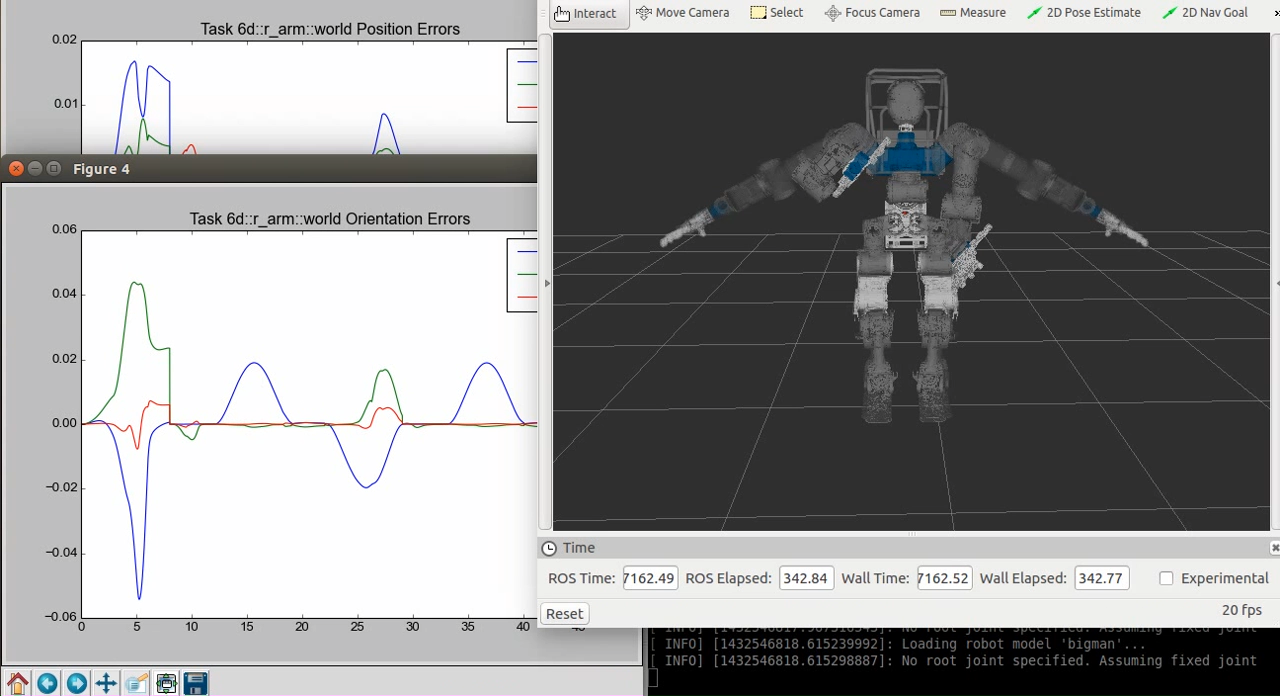
\includegraphics[width=0.7\textwidth]{images/software/previewer} 
\caption{The phantom model is superposed to the robot model to show the motion that the robot will perform. Plot of the trajectories are automatically generated by the previewer} 
\label{fig:previewer}
\end{figure*}

The success of the action will be determined according to the settings of the previewer, and the specified duration of the preview action. In fact, a user can decide to preview an action partially, and get results from that partial preview of an entire trajectory, or preview an action till convergence is detected. The success is determined when no error conditions where raised during preview, and one of the following convergence conditions is true at the end of the preview action:
\begin{itemize}
\item Cartesian error is small
\item Cartesian error is small and not decreasing
\item Cartesian error is small, not decreasing, and joint velocities are below a user-defined threshold (null-space tasks converged) 
\end{itemize}

\begin{table}[hbt]
   \small
   \begin{center}
   \begin{tabular}{| >{\centering\arraybackslash}m{2.3in} | >{\centering\arraybackslash}m{0.5in} | >{\centering\arraybackslash}m{3in} |}
   \hline
   \textbf{Constant} & \textbf{Default Value} & \textbf{Meaning} \\\hline
   \cline{1-3}
   \footnotesize{\texttt{TRAJECTORIES\_EXPIRED\_SAFETY\_MARGIN}}           & $1.5$   & \shortstack{when previewing for an infinite time, stop \\ \footnotesize{\texttt{if t >= longest\_task\_duration * safety\_margin}}} \\\hline
   \footnotesize{\texttt{UPDATE\_ERR\_STATS\_WINDOW\_SIZE\_IN\_SECS}} & $0.1$    & \shortstack{set the time window of the moving average filter \\ for the error statistics} \\\hline
   \footnotesize{\texttt{PREVIEWER\_CHECK\_MAX\_RETRIES}}                  & $3$     & if \texttt{solve()} fails, retry for a maximum of \footnotesize{\texttt{MAX\_RETRIES}} \\\hline
   \footnotesize{\texttt{TRAJ\_BINDING\_MAXIMUM\_ALLOWED\_ERR}}           & $5\times10^{-2}$  & \shortstack{maximum allowed Cartesian error, in norm, \\ during task execution} \\\hline
   \footnotesize{\texttt{TRAJ\_BINDING\_CONVERGENCE\_TOLERANCE}}           & $5\times10^{-4}$  & threshold value for Cartesian error norm convergence \\\hline
   \end{tabular}
   \end{center}
   \caption{Previewer default configuration. Values used for previewing motions on an adult-sized humanoid robot.}
   \label{table:previewer_constants}
\end{table}

\paragraph{Logging and Plotting}
\label{par:logging-plotting}
YARP provides a functionality for plotting and logging signals, such as joint velocities, joint torques and force/torque sensor readings.
The same can be said about ROS, and since the software architecture used by the WALKMAN team comprised a mix between the two middlewares, both could be used to store and visualize crucial data during robot operation. Still, the facilities these middlewares provide expect developers to \emph{publish} all the data that needs to be stored/visualized, resulting in a large overhead which often can become unbearable for continuous logging by the onboard control pc, especially when, together with the basic sensor data, we are interested in logging and visualizing statistics about the control algorithm performance.

For this reason, a toolkit to easily store and plot data has been implemented in OpenSoT.
The logging and ploting framework is based on the idea of \emph{flushers} and \emph{plotters}. 
The \emph{logger} is created by stacking a list of flushers, each of them taking care of serializing the data to be saved on a text file. Each flusher can be instantiated with additional information regarding the data that is storing, e.g. joint names and unit of measurements.
A plotter can be created that plots the logged data, a subset of the data, or the result of an operation executed on the stored data (such as norm, multiplication between compatible data fields and filtering), and in general a plot will consist of several plotters taking care of visualizing the data saved by a logger. The plotter can make use of the semantic information about the data form the flushers, so that many aspects of plot generation can be automated, e.g. legend generation.
The framework allows to automatically store and plot data relative to Tasks, Constraints, robot sensors data, and raw data (scalars, vectors, matrices); the user can easily write additional flushers and plotters for arbitrary complex data structures, extend the basic flushers in order to store data using different data formats, or extend the basic plotters in order to plot using different plotting environments.
At the time the flushers and the plotters all use python data and plotting functionalities, allowing the plotters to work even on the control pc of the robot where \emph{Matlab} is not available.

\section{Conclusions}
While in previous section the theoretical foundations of the high level control framework are addressed and presented together with a large set of experiments, in this section the API, the software infrastructure and the utilities ecosystem has been detailed, with the intent of demonstrating the richness of features of our high level control scheme.
Statistics and best-practices used in the WALKMAN team have been presented as part of the work for the DRC competition. Lastly, the simulation, middleware and component model used by the team has been presented as a fundamental scaffolding of the work of the team and as a means of organizing the work of the team.